%
% $RCSfile: cybernetics_oriented_interpreter.tex,v $
%
% Copyright (c) 2001-2004. Christian Heller. All rights reserved.
%
% No copying, altering, distribution or any other actions concerning this
% document, except after explicit permission by the author!
% At some later point in time, this document is planned to be put under
% the GNU FDL license. For now, _everything_ is _restricted_ by the author.
%
% http://www.cybop.net
% - Cybernetics Oriented Programming -
%
% http://www.resmedicinae.org
% - Information in Medicine -
%
% @author Christian Heller <christian.heller@tuxtax.de>
%

\subsection{Cybernetics Oriented Interpreter}
\label{cybernetics_oriented_interpreter_heading}

The CYBOL language described in section \ref{cybernetics_oriented_language_heading}
is just another form of storing knowledge. It can therefore also be called a
\emph{Knowledge Modelling Language}.

\begin{figure}[ht]
    \begin{center}
        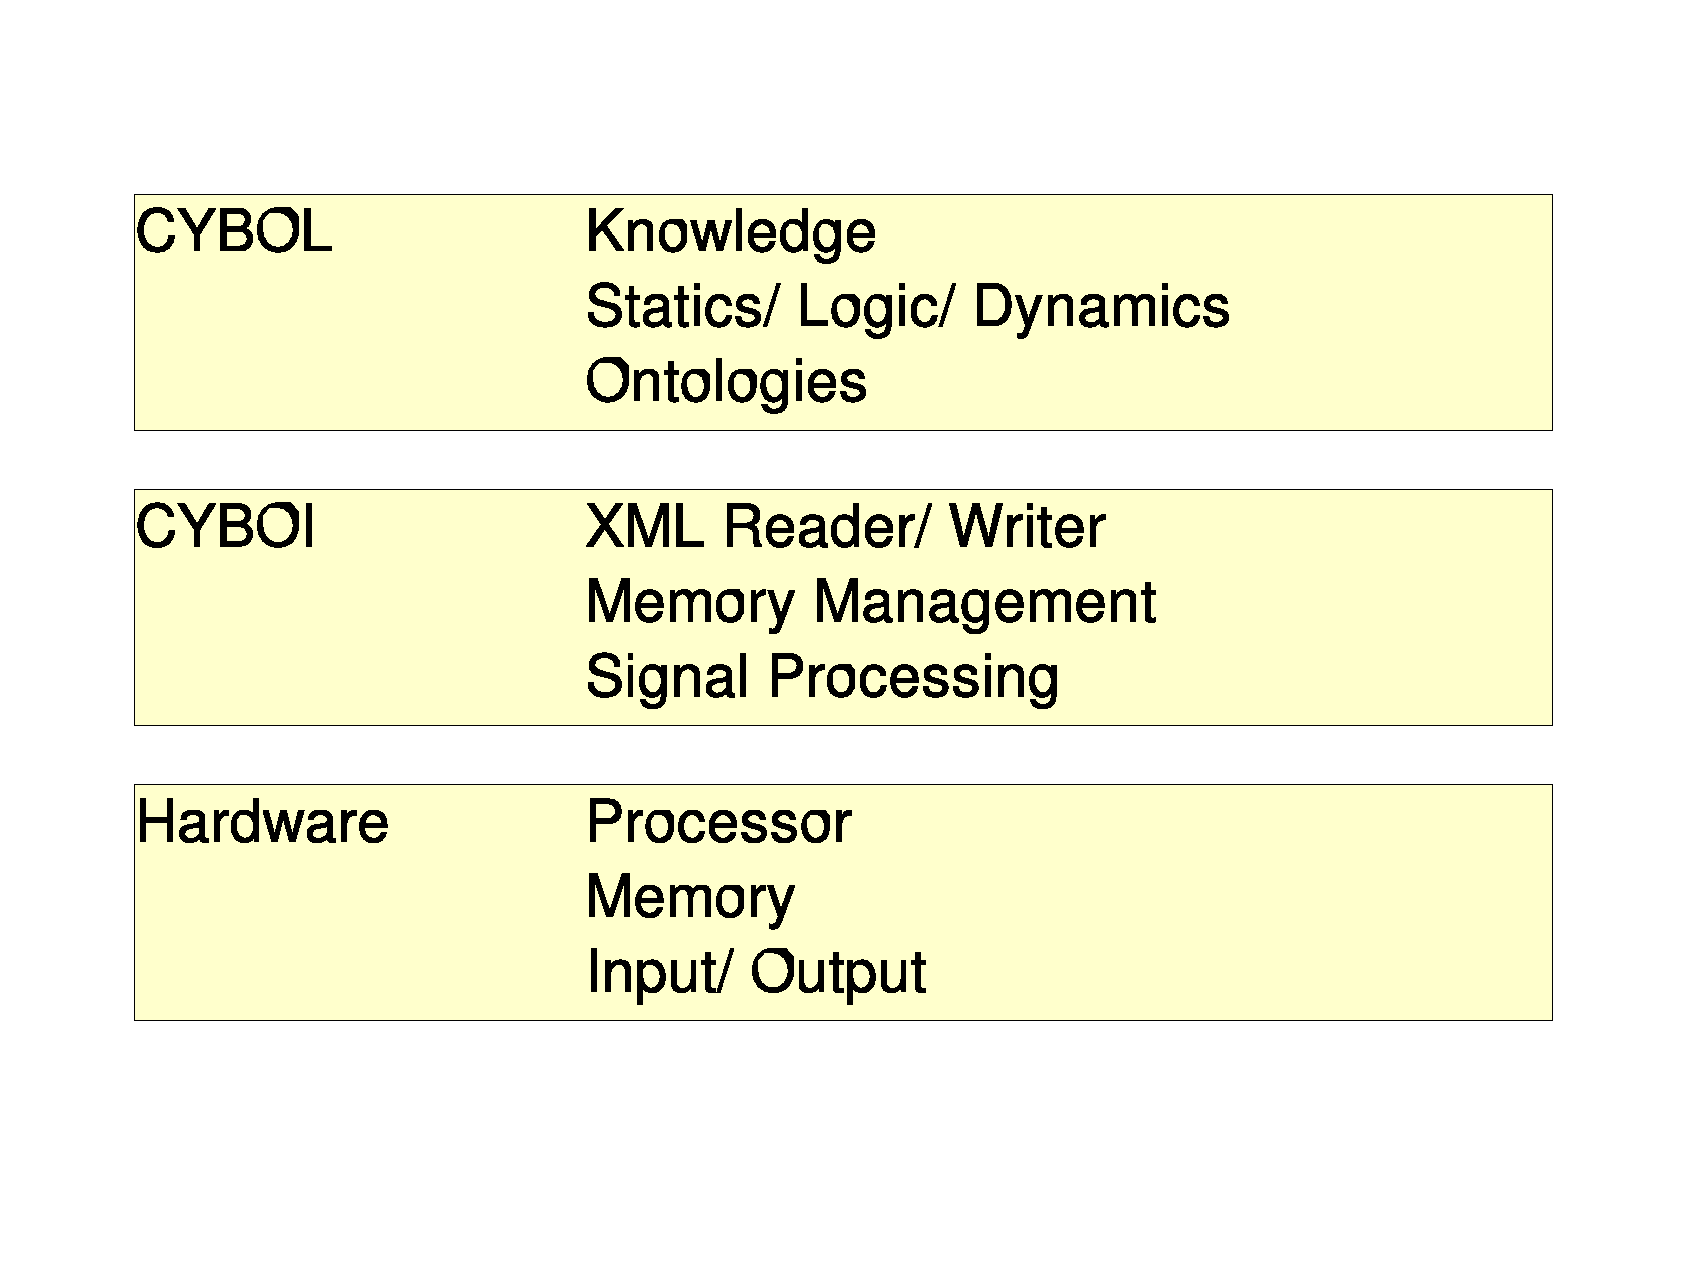
\includegraphics[scale=0.3]{vector/hardware_connection.eps}
        \caption{CYBOI as Interface between CYBOL and Hardware}
        \label{hardware_connection_figure}
    \end{center}
\end{figure}

When CYBOL files contain the knowledge that
defines a system, a counterpart is needed to execute that system on computer
hardware. The \emph{Cybernetics Oriented Interpreter} (CYBOI) is able to handle
this task (figure \ref{hardware_connection_figure}).
CYBOI is written in the C programming language and currently supports the
\emph{Linux} \emph{Operating System} (OS) only. It represents, so to say, the
interface between operating instructions of the computer hardware and system
models defined in CYBOL.

CYBOI is responsible for managing any kind of hardware communication, that is
input, output, memory access and processor instruction calls. CYBOI Signals can
be assigned priorities, a language (protocol) to communicate with other systems
and they are processed by one single loop (figure \ref{cyboi_figure}). Also,
there is only one single container structure which CYBOI uses to dynamically
store knowledge. It such avoids the known problems with container inheritance
\cite{javaiaq}. Following \emph{Euclidian Geometry}, multi-dimensional
\emph{Models} consist of maps; two-dimensional \emph{Maps} consist of arrays;
one-dimensional \emph{Arrays} represent and manage an area in the computer memory.

\begin{figure}[ht]
    \begin{center}
        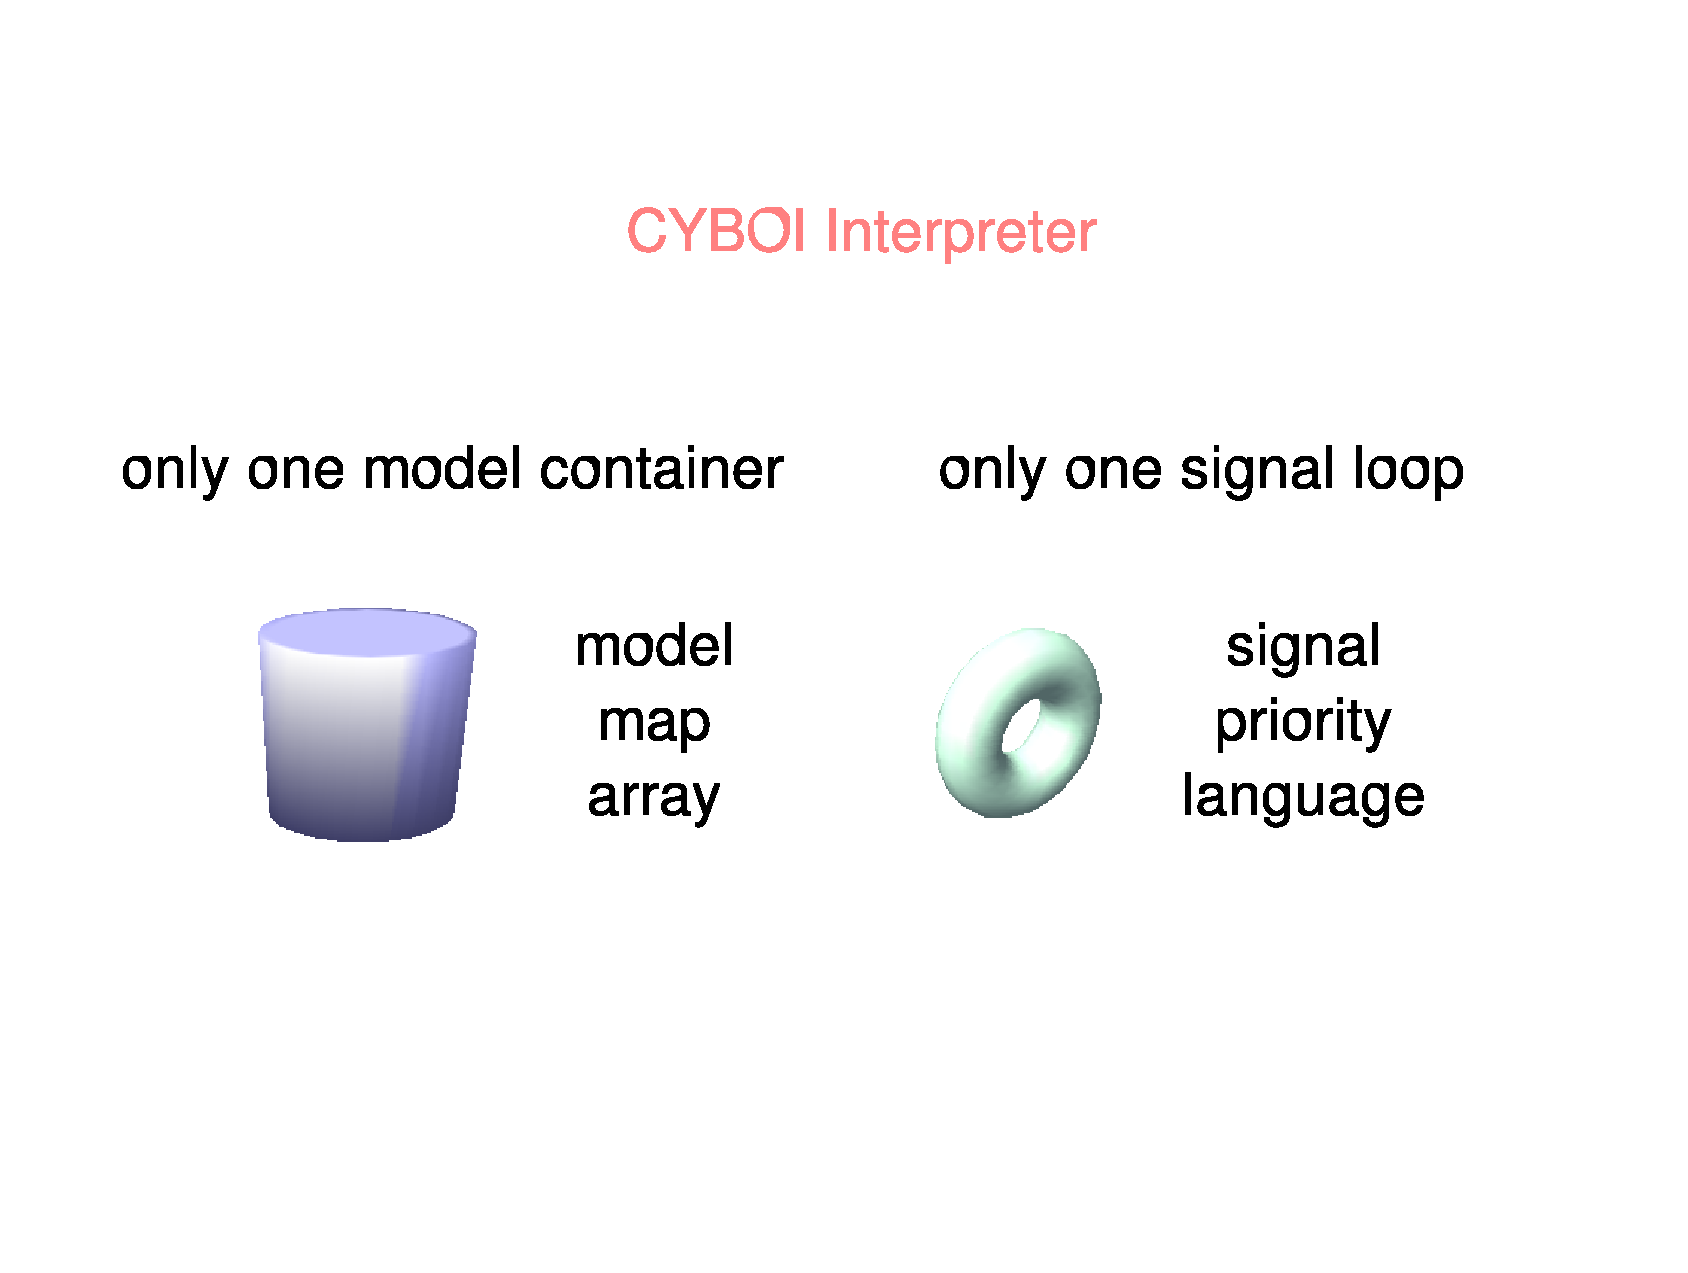
\includegraphics[scale=0.3]{vector/cyboi.eps}
        \caption{CYBOI Model Container and Signal Loop}
        \label{cyboi_figure}
    \end{center}
\end{figure}

The more hardware driving functionality CYBOI implements, the more it develops
towards an operating system -- with one difference to current OS: It is free of
any configuration information but knows how to \emph{handle} knowledge.
